\lecture{7}{February 1, 2017}{Yassir M'rabet, Thibaud Canale}
\section{Introduction}
This final lesson is about how to use game theory in engineering. The goal of game theory is to optimize a function that is unknown, in many cases we named it the utility function.\\*
We will see that in order to design a system that we want to reach an optimum configuration, we need to deploy agents that can choose between a set of strategies, each giving a certain payoff. Agents will keep changing their actions in order to increase their utilities and it will make them reach an optimal state which is an equilibrium. 
\section{Potential Games}
We want to design a game that converges by dynamics to an equilibrium. We introduce the notion of Potential Games. A game is said to be a potential game if the incentive of all players to change their strategy can be expressed using a single global function called the potential function. When an agent will change its state to increase its utility, the potential function associated to the system will also increase. And in potential games the existence of pure strategy Nash equilibrium is guaranteed, and multiple Nash equilibrium may exist. We only need to choose the potential function that satisfies: 
\begin{equation}
\exists \varphi(\underset{-}{a}) \qquad / \qquad  U_i(a'_i,\underset{-}{a_{-i}})-U_i(a_i,\underset{-}{a_{-i}})=\varphi(a'_i,\underset{-}{a_{-i}})-\varphi(a_i,\underset{-}{a_{-i}}) \qquad \forall a'_i,a_i, \underset{-}{a_{-i}}  \qqad \forall i
\end{equation}
The non-trivial assumption of the equation is that it should be true for all agents.\\*
We will look at the implications of equation (1) in the following. Let us consider a set of agents $a_i $ that can choose to change their state. $a_1 $ will first change its state: \\*
\\*
\hspace*{20pt} $a_1^{(0)},a_2^{(0)},a_3^{(0)}...a_N^{(0)}$ \hspace*{15pt} to \hspace*{15pt} $a_1^{(1)},a_2^{(0)},a_3^{(0)}...a_N^{(0)}$ \\* \\*
It means that a1 increases its utility while it decided to change its state. \\* \\*
\hspace*{20pt} $U1(a_1^{(1)},a_2^{(0)},a_3^{(0)}...a_N^{(0)})$  \textgreater $U1(a_1^{(0)},a_2^{(0)},a_3^{(0)}...a_N^{(0)})$  \\* \\*
Which means, from equation (1), that a1 increased the potential of the system by changing state. \\* \\*
\hspace*{20pt} $\varphi(a_1^{(1)},a_2^{(0)},a_3^{(0)}...a_N^{(0)})$ \textgreater $\varphi(a_1^{(0)},a_2^{(0)},a_3^{(0)}...a_N^{(0)})$ \\* \\*
Now agent a2 changes its state, we get \hspace{5pt} $a_1^{(1)},a_2^{(1)},a_3^{(0)}...a_N^{(0)}$
\\* 
It means that its action changed the total utility positively: \\*
$U2(a_1^{(1)},a_2^{(1)},a_3^{(0)}...a_N^{(0)})$ \textgreater $U2(a_1^{(1)},a_2^{(0)},a_3^{(0)}...a_N^{(0)})$ \\*
Note that we do not know how the utility of agent 1 changed $U1(a_1^{(1)},a_2^{(1)},a_3^{(0)}...a_N^{(0)})$ ? $U1(a_1^{(1)},a_2^{(0)},a_3^{(0)}...a_N^{(0)})$  \\*
But all what matter at this state is the variation of the potential function, and we know by the definition of a potential game that it increased: \\*
$\varphi(a_1^{(1)},a_2^{(1)},a_3^{(0)}...a_N^{(0)})$ \textgreater $\varphi(a_1^{(1)},a_2^{(0)},a_3^{(0)}...a_N^{(0)})$ \\*
A question that we can ask ourselves is do the dynamic stop ? \\*
At this point we know that if the dynamic stop we are in a pure strategy Nash Equilibrium. The condition for the system to stop is that the space of possible strategies should be finite to say that the dynamics will stop. Namely the function of potential $\varphi$ should have a finite number of values that it can take. 
\section{Designing a Game}
We know the condition that must be satisfied when choosing the utility function in order to be in the case of potential games, which is choosing a function where if each agent changes its state to increase its utility, it should cause an increase in the potential function associated to the utility function. \\*
A good way to make sure that the condition will be satisfied is to choose the potential function to be the same as the utility one $\varphi=W$ therefore the game can be expressed as: \\*
\begin{equation}
\underset{a_i \in A_i \forall i }{Maximize} \qquad W(a_1,a_2,a_3,...,a_N )
\end{equation}
The total utility is then computed by: 
\begin{equation}
U_i(a'_i,a_{-i})-U_i(a_i,a_{-i})=W(a'_i,a_{-i})-W_i(a_i,a_{-i})
\end{equation}
To be able to compute values of the utility we need to add that at a given point the utility is null, it comes as a referential for the computation. The computation of a difference between potential only include the final state and the initial one, this is why we need to have an information about the first state. \\* 
We put \hspace{5pt} $U_i(a_i^{0},a_{-i})=0$ \hspace{5pt} $ \forall a_{-i}$ \\*
\section{An Application}
We will consider the problem of an area that needs to be covered by robots that sense a specific range. In this area there are risky places where a fire could start. We therefore need to put the robots in the area and then the robots will keep changing until reaching a configuration where risky places are well covered.
\begin{figure}[!htb]
   \centering
    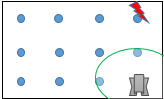
\includegraphics{C1}
    \caption{Illustration of the problem}
\end{figure}
\\*
We say that: \\
$A_i$ is the set of positions. \\
$P(\underset{-}{s})$ is the probability that the fire occurs at $\underset{-}{s}.$ \\
$D_i(a_i,\underset{-}{s})$ is the probability that robot i at position $a_i$ detects the fire in $\underset{-}{s}.$ \\
Putting these variable, we will define the function that we want to maximize, which is the probability that the robot senses the fire and that a fire occurs:
 \\*
\begin{equation}
W(\underset{-}{a})=\sum\limits_{\underset{-}{s}}(1-\prod\limits_{i}(1-D_i(a_i,\underset{-}{s})))
\end{equation}
\\*
Robots will compute their utility following the equation:
\begin{equation}
U_i(a_i,a_{-i})=U_i(a^{0},a_{-i})+W(a_i,a_{-i})-W_i(a^{0},a_{-i})
\end{equation}
Where: 
$U_i(a^{0},a_{-i})=0$  \\
From (4) equation (5) becomes:
\begin{equation}
U_i(a_i,a_{-i})=\sum\limits_{\underset{-}{s}}P(\underset{-}{s})[1-\prod\limits_{j\neq i}(1-D_j(a_j,\underset{-}{s}))(1-D_i(a_i,\underset{-}{s}))-1+\prod\limits_{j\neq i}(1-D_j(a_j,\underset{-}{s}))(1-D_i(a^{0},\underset{-}{s}))]
\end{equation}
By looking at this equation we could think that a robot needs to know the position of all the other robots in order to compute its utility, but actually it is not the case, there are places not affected by the sensing of the robots, they will naturally not appear in the equation, we will modify the limits of the sum:
\begin{figure}[!htb]
   \centering
    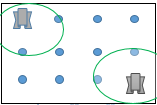
\includegraphics{C2}
    \caption{Interaction model between robots}
\end{figure}
\\*
The resultant equation: 
\begin{align*}
U_i(a_i,a_{-i})=\sum\limits_{\underset{-}{s} \in N(a_i)}P(\underset{-}{s})[1-\prod\limits_{j\neq i}(1-D_j(a_j,\underset{-}{s}))(1-D_i(a_i,\underset{-}{s}))-1+\prod\limits_{j\neq i}(1-D_j(a_j,\underset{-}{s}))(1-D_i(a^{0},\underset{-}{s}))] \\
-\sum\limits_{\underset{-}{s} \in N(a_i)}P(\underset{-}{s})[1-\prod\limits_{j\neq i}(1-D_j(a_j,\underset{-}{s}))(1-D_i(a^{0},\underset{-}{s}))-1+\prod\limits_{j\neq i}(1-D_j(a_j,\underset{-}{s}))(1-D_i(a_i,\underset{-}{s}))]
\end{align*}
Another remark is that, as we said, we only look at the sensing region at the initial state and the final one, the equation will therefore not contain all the places where the robot that changes its state is, we will write the equation again but specifying this region by modifying the limit of the product: 
\begin{align*}
U_i(a_i,a_{-i})=\sum\limits_{\underset{-}{s} \in N(a_i)}P(\underset{-}{s})[1-\prod\limits_{j/\underset{-}{s} \in N(a_j)}(1-D_j(a_j,\underset{-}{s}))(1-D_i(a_i,\underset{-}{s}))-1+\prod\limits_{j/\underset{-}{s} \in N(a_j)}(1-D_j(a_j,\underset{-}{s}))(1-D_i(a^{0},\underset{-}{s}))] \\ -\sum\limits_{\underset{-}{s} \in N(a_i)}P(\underset{-}{s})[1-\prod\limits_{j /\underset{-}{s} \in N(a_j)}(1-D_j(a_j,\underset{-}{s}))(1-D_i(a^{0},\underset{-}{s}))-1+\prod\limits_{j/\underset{-}{s} \in N(a_j) i}(1-D_j(a_j,\underset{-}{s}))(1-D_i(a_i,\underset{-}{s}))]
\end{align*}
We rearrange the equation: 
\begin{align*}
U_i(a_i,a_{-i})=\sum\limits_{\underset{-}{s} \in N(a_i)}P(\underset{-}{s})[\prod\limits_{j/\underset{-}{s} \in N(a_j)}(1-D_j(a_j,\underset{-}{s}))(D_i(a_i,\underset{-}{s})-D_i(a^{0},\underset{-}{s}))] \\ -\sum\limits_{\underset{-}{s} \in N(a_i)}P(\underset{-}{s})[\prod\limits_{j/\underset{-}{s} \in N(a_j)}(1-D_j(a_j,\underset{-}{s}))(D_i(a^{0},\underset{-}{s})-D_i(a_i,\underset{-}{s}))]
\end{align*}
The result of this equation will give the agent the information on the position it should got to. An output of the computation could be that a place is risky but already well covered by agents, and an agent's increase of utility will be to go to another place not as risky but less covered. \\
We saw that at first it appears to be a centralized problem where an agent needs to know about the position of all agents to compute its utility, but finally an agent only needs to know about its neighbors, which puts the solution as a distributed one.